\documentclass[10pt]{beamer}

\usetheme[progressbar=frametitle]{metropolis}
\definecolor{ag-maroon}{RGB}{80,0,0}
\definecolor{ag-maroon2}{RGB}{60,0,0}
\definecolor{ag-blue}{RGB}{0,60,113}
\definecolor{ag-odgreen}{RGB}{91,98,54}
\definecolor{ag-brown}{RGB}{116,79,40}
\definecolor{ag-tan}{RGB}{153,133,66}
\definecolor{ag-beige}{RGB}{214,210,196}
\definecolor{ag-white}{RGB}{246,246,246}
\definecolor{ag-black}{RGB}{0,0,0}
\definecolor{ag-light-black}{RGB}{20,20,20}

\setbeamercolor{background canvas}{fg=ag-white}
\setbeamercolor{normal text}{fg=ag-black}
\setbeamercolor{alerted text}{fg=ag-tan}
\setbeamercolor{example text}{fg=ag-light-black}

\setbeamercolor{frametitle}{bg=ag-blue}
\setbeamercolor{progress bar}{fg=ag-maroon}
\setbeamercolor{title separator}{fg=ag-blue}
\setbeamercolor{progress bar in head/foot}{fg=ag-tan}
\setbeamercolor{progress bar in section page}{fg=ag-tan}


\usepackage{appendixnumberbeamer}

\usepackage{booktabs}
\usepackage[scale=2]{ccicons}

\usepackage{pgfplots}
\usepgfplotslibrary{dateplot}

\usepackage{xspace}
\newcommand{\themename}{\textbf{\textsc{metropolis}}\xspace}

\usepackage{amsfonts,amsmath,amssymb,amsthm}
\usepackage{graphicx}
\usepackage[export]{adjustbox} % For advanced image adjustments
\usepackage{caption}           % For captions (optional)

% \graphicspath{{../figures}}
\usepackage{tikz}
\usetikzlibrary{arrows.meta, positioning, shapes, intersections, calc, overlay-beamer-styles}
\usepackage{tcolorbox}


%%%%%%%%%%%%%%%%%%%
% Custom commands

\newcommand{\bb}[1]{\boldsymbol{#1}}
\newcommand{\tr}{^{\intercal}}
\newcommand{\R}{\mathbb{R}}
\newcommand{\E}{\mathbb{E}}
\newcommand{\argmax}{\arg\,\max}
\newcommand{\argmin}{\arg\,\min}
\newcommand{\Fcal}{\mathcal{F}}

%%%%%%%%%%%%%%%%%%
% TITLE AREA
\title{Generalized Alpha-Beta Divergence, its Properties and Associated Entropy}
% \subtitle{A Robust Singular Value Decomposition Technique}
% \date{\today}
\date{}
\author{Subhrajyoty Roy}
\institute{Research Fellow, Interdisciplinary Statistical Research Unit\\
    Indian Statistical Institute, Kolkata, India\\
    \begin{flushright}
        May 19, 2025\\
        ICORS 2025, Stresa, Italy
    \end{flushright}
}
% \titlegraphic{\hfill
\includegraphics[height=1.5cm]{logo.pdf}}


\makeatletter
\let\save@measuring@true\measuring@true
\def\measuring@true{%
  \save@measuring@true
  \def\beamer@sortzero##1{\beamer@ifnextcharospec{\beamer@sortzeroread{##1}}{}}%
  \def\beamer@sortzeroread##1<##2>{}%
  \def\beamer@finalnospec{}%
}
\makeatother

\begin{document}

\maketitle

\begin{frame}{Co-authors}
\begin{columns}[c] % 'c' for vertical centering

  \column{0.33\textwidth}
  \centering
  \adjincludegraphics[height=3cm,clip]{./SupratikBasu.jpg}
  
  \vspace{0.5em}
  \small Supratik Basu

  \column{0.33\textwidth}
  \centering
  \adjincludegraphics[height=3cm,clip]{./AbhikGhosh.jpg}
  
  \vspace{0.5em}
  \small Abhik Ghosh

  \column{0.33\textwidth}
  \centering
  \adjincludegraphics[height=3cm,clip]{./AyanBasu.jpg}
  
  \vspace{0.5em}
  \small Ayanendranath Basu

\end{columns}

\end{frame}


\begin{frame}{Statistical Divergence}
    A \textbf{statistical divergence} $d: \Fcal \times \Fcal \rightarrow [0, \infty)$ such that $d(f, g) = 0$ if and only if $f = g$ almost surely.

    \pause

    Weaker than a metric.
    \begin{enumerate}
        \item $d(f, g)$ and $d(g, f)$ may be different.
        \item Usually no relationship between $d(f, g)$ and $d(f, h) + d(h, g)$.
    \end{enumerate}

    \pause
    You can extend for \textbf{sub-densities}
    \begin{equation*}
        \Fcal^\ast := \left\{ f : f \geq 0, \int fd\mu \leq 1  \right\}.
    \end{equation*}
\end{frame}

\begin{frame}{Minimum divergence estimation}

    Given a statistical model $\{ f_\theta : \theta \in \Theta \}$ and a divergence measure $d(\cdot, \cdot)$ between distributions, the \textbf{minimum divergence estimator} (MDE) of $\theta$ minimizes the divergence between a ``proxy'' data density $g$ and the model density $f_\theta$:

    \begin{equation*}
        \theta^\ast = \arg\min_{\theta \in \Theta} d(g, f_\theta).
    \end{equation*}

    \pause
    \vspace*{2em}

    \begin{columns}[c]

    \column{0.6\textwidth}
    \centering
    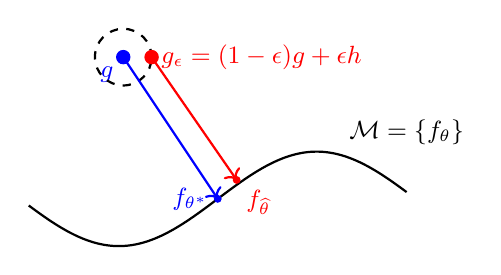
\begin{tikzpicture}[scale=1.2, every node/.style={font=\small}]
        % Model manifold
        \draw[thick, smooth, samples=100, domain=-2:2] plot (\x, {0.5*sin(1.5*\x r)});
        \node at (2,0.7) {\( \mathcal{M} = \{ f_\theta \} \)};

        % Node for true distribution g
        \filldraw[blue] (-1,1.5) circle (2pt) node[below left] {\( g \)};
    
        % Draw contamination ball
        \draw[thick, dashed] (-1,1.5) circle (0.3cm);
            
        % Projection from g to manifold (theta*)
        \filldraw[blue] (0,0) circle (1pt) node[left] {\( f_{\theta^\ast} \)};
        \draw[->, thick, blue] (-1,1.5) -- (0,0);
    
        % Contaminated point (tilde g)
        \filldraw[red] (-0.7,1.5) circle (2pt) node[right] {$g_\epsilon = (1-\epsilon) g + \epsilon h$};
        \draw[->, thick, red] (-0.7,1.5) -- (0.2, 0.2);
        \filldraw[red] (0.2,0.2) circle (1pt) node[below right] {$f_{\widehat{\theta}}$};
    \end{tikzpicture}

    \column{0.4\textwidth}
    \pause

    The choice of divergence $d(\cdot, \cdot)$ controls the curvature of these geodesic lines.
    \end{columns}

\end{frame}


\begin{frame}{Useful divergences for Robust Estimation}
Several divergences have been proposed to balance \textbf{efficiency} and \textbf{robustness}:

\begin{itemize}
    \item \textbf{Density Power Divergence (DPD)}~\cite{basu1998robust}:
    \[
    d_{DPD}^{\alpha}(g, f) = \int f^{1+\alpha} - \left(1 + \frac{1}{\alpha}\right) \int g f^\alpha + \frac{1}{\alpha} \int g^{1+\alpha}.
    \]

    \vspace{0.5em}

    \item \textbf{Log-Density Power Divergence (LDPD)}~\cite{jones2001comparison}:
    \[
    d_{\text{LDPD}}^{\alpha}(g, f) = \log \int f^{1+\alpha} - \left(1+\frac{1}{\alpha}\right) \log \int g f^\alpha + \frac{1}{\alpha} \log \int g^{1+\alpha}.
    \]

    \vspace{0.5em}

    \item \textbf{Bridge Divergence}~\cite{kuchibhotla2019bridge}
    \begin{multline*}
        d_{\text{BD}}^{\alpha,c_1,c_2}(g, f) = \log\left( c_1 + c_2 \int f^{1+\alpha} \right)
        - \left(1+\frac{1}{\alpha}\right) \log \left( c_1 + c_2 \int g f^\alpha \right) \\
        + \frac{1}{\alpha} \log \left( c_1 + c_2 \int g^{1+\alpha}\right).        
    \end{multline*}
\end{itemize}
\end{frame}

\begin{frame}{Useful divergences for Robust Estimation}
    \begin{itemize}
        \item \textbf{S-divergence family}~\cite{sdiv}:
        \[
        d_{SD}^{\alpha,\lambda}(g, f) = \frac{1}{A} \int f^{1+\alpha} - \frac{1+\alpha}{AB} \int f^B g^A + \frac{1}{B} \int g^{1+\alpha},
        \]
        where \( A = 1 + \lambda(1-\alpha) \), \( B = 1 + \alpha - \lambda(1-\alpha) \).
        \item \textbf{Logarithmic S-divergence family}~\cite{maji2016logarithmic}:
        \[
        d_{LSD}^{\alpha,\lambda}(g, f) = \frac{1}{A} \log\left( \int f^{1+\alpha} \right) - \frac{1+\alpha}{AB} \log\left( \int f^B g^A \right) + \frac{1}{B} \log\left( \int g^{1+\alpha} \right),
        \]
        where \( A = 1 + \lambda(1-\alpha) \), \( B = 1 + \alpha - \lambda(1-\alpha) \).
    \end{itemize}
\end{frame}




\begin{frame}{Generalized Alpha-Beta Divergence}
    We define the generalised alpha-beta divergence (GABD) as
    \begin{multline*}
        d_{GAB}^{(\alpha,\beta),\psi}(f, g) = \dfrac{1}{\beta(\alpha+\beta)}\psi\left( \int f^{\alpha+\beta} \right) \\
        - \frac{1}{\alpha\beta} \psi\left( \int f^\alpha g^\beta \right) + \frac{1}{\alpha(\alpha+\beta)}\psi\left( \int g^{\alpha+\beta} \right),
    \end{multline*}
    \noindent where $\psi$ is a suitable function.

    If $\psi$ is continuously differentiable, then we can define the cases $\alpha = 0, \beta = 0, (\alpha+\beta) = 0$ by taking corresponding limits.

    \pause

    \begin{itemize}
        \item $\psi(x) = x$, gives you super divergence.\\
        \item $\psi(x) = x, \beta = 1$ gives you density power divergence.\\
        \item $\psi(x) = \log(x)$, gives you logarithmic super divergence.\\
        \item $\psi(x) = \frac{1}{\gamma} x^\gamma$, gives you $(\phi,\gamma)$-divergence.
    \end{itemize}
    \pause
    \textcolor{red}{Does every $\psi(\cdot)$ make it a divergence?}
    % No, because if \psi() makes it a divergence, -\psi() does not work.
\end{frame}

\begin{frame}{Key Result: Necessary and Sufficient Conditions}

    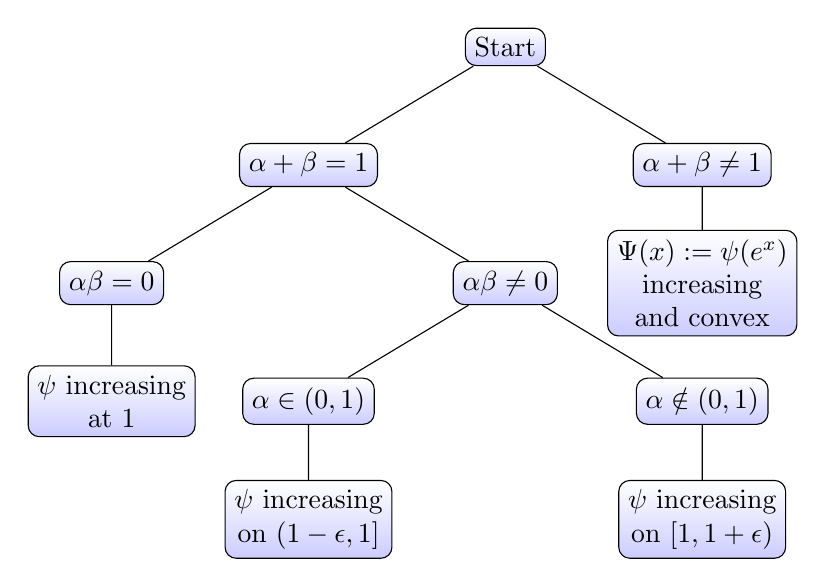
\begin{tikzpicture}[>=stealth, level distance=1.5cm, sibling distance=5cm,
      every node/.style = {shape=rectangle, rounded corners,
        draw, align=center, top color=white, bottom color=blue!20}]
    
      \node {Start}
        child { node {\( \alpha + \beta = 1 \)}
          child { node {\( \alpha\beta = 0 \)}
            child { node {\( \psi \) increasing \\ at \( 1 \)} }
          }
          child { node {\( \alpha\beta \neq 0 \)}
            child { node {\( \alpha \in (0,1) \)}
              child { node {\( \psi \) increasing\\ on \( (1-\epsilon, 1] \)} }
            }
            child { node {\( \alpha \notin (0,1) \)}
              child { node {\( \psi \) increasing\\ on \( [1, 1+\epsilon) \)} }
            }
          }
        }
        child { node {\( \alpha + \beta \neq 1 \)}
          child { node { $\Psi(x) := \psi(e^x)$\\ increasing\\ and convex} }
        };
    \end{tikzpicture}
\end{frame}


\begin{frame}{Recipe for new divergences}
    \begin{enumerate}
        \item Start with any nonnegative function $f$.
        \item Define, $F(x) = \int_{-\infty}^x f(t)dt$. If $f$ is density, $F$ is the cdf.
        \item Define $\psi(x) = \int_{-\infty}^{\log(x)} F(u)du$.
    \end{enumerate}

    \pause

    Some examples are:
    \begin{itemize}
        \item LSD when $f = \delta(0)$.
        \item $(\phi,\gamma)$-divergence ($x \leq 1$) when $f$ is the density of $\exp(\gamma)$.
        \item Bridge divergence when $f$ is $\text{Logistic}(\log(c_1/c_2), 1)$.
    \end{itemize}

\end{frame}

\begin{frame}{New divergences}
    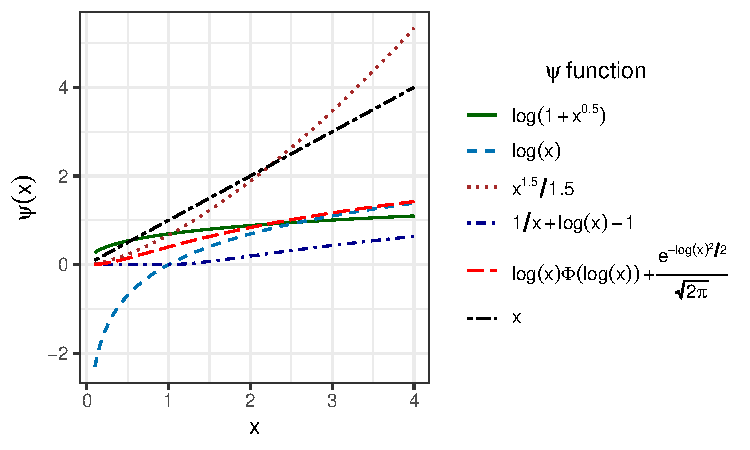
\includegraphics[width = \textwidth]{./gab-psi-functions.pdf}
\end{frame}

\begin{frame}{Special cases}
    \begin{itemize}
        \item In location models, all MGABDE are equivalent, i.e., $d_{GAB}^{(\alpha,\beta),\psi_1}(f, g) = h(d_{GAB}^{(\alpha,\beta),\psi_2}(f,g))$ for some monotonic function $h$.
        \pause
        \item For a density $f$, let $f^{[\alpha]}(x) = f^\alpha(x) / \int f^\alpha(u)du$. When $\beta = 0, \alpha \neq 0$,
        \begin{multline*}
            d_{GAB}^{(\alpha,0),\psi}(f, g)
            = \frac{\psi'(\int f^\alpha) \int f^\alpha}{\alpha^2}\left( \textcolor{blue}{d_{KL}(f^{[\alpha]}, g^{[\alpha]})} + \ln\left( \frac{\int f^\alpha}{\int g^\alpha} \right) \right)\\
            - \psi\left(\int f^\alpha\right) + \psi\left( \int g^\alpha \right)
        \end{multline*}
        \pause
        \item When $\alpha + \beta = 1, \alpha \notin \{0, 1\}$,
        \begin{equation*}
            d_{GAB}^{(\alpha,1-\alpha),\psi} = \frac{1}{\alpha(1-\alpha)} \left[ \psi(1) - \psi\left( \textcolor{blue}{d_{PD, \alpha}(f, g)} + \text{constant} \right) \right]
        \end{equation*}
    \end{itemize}
\end{frame}

\begin{frame}{Properties}

    \begin{itemize}
        \item \textbf{Duality}: $d_{GAB}^{(\alpha,\beta),\psi}(f, g) = d_{GAB}^{(\beta,\alpha),\psi}(g, f)$.
        \item \textbf{Scaling}: $d_{GAB}^{(\alpha,\beta),\psi}(cf, cg) = d_{GAB}^{(\alpha,\beta), \psi(c^{\alpha+\beta} \cdot)}(f, g)$.
        \item \textbf{Zooming}: $d_{GAB}^{(\alpha,\beta),\psi}(f^\tau, g^\tau) = \tau^2 d_{GAB}^{(\tau\alpha,\tau\beta),\psi}(f, g)$.
    \end{itemize}

    \pause

    % see if you can make a blue box
    \begin{theorem}[Approximate Pythagorean Identity]
        \begin{enumerate}
            \item Let $\psi$ be continuously differentiable.
            \item $\alpha\beta(\alpha+\beta) \neq 0$.
            \item $g_\epsilon^\alpha = (1-\epsilon)g^\alpha + \epsilon \delta^\alpha$.
        \end{enumerate}
        Then, 
        \begin{multline*}
            d_{GAB}^{(\alpha,\beta),\psi}(g_\epsilon, f)
            = d_{GAB}^{(\alpha,\beta),\psi}(g_\epsilon, g) 
            + d_{GAB}^{(\alpha,\beta),\psi}(g, f) 
            \\
            + O_{\psi}\left( \epsilon \right) + O_{\psi}\left( \ln(1-\epsilon) \right)
        \end{multline*}
    \end{theorem} 
\end{frame}

\begin{frame}{Generalized Alpha-Beta Entropy}
   \begin{definition}[GAB Entropy]
       \begin{equation*}
           \varepsilon_{GAB}^{(\alpha,\beta),\psi}(f) = -\frac{1}{\beta}\left[ \frac{\psi(\int f^{\alpha+\beta})}{\alpha+\beta} - \frac{\psi(\int f^\alpha)}{\alpha} \right].
       \end{equation*}
   \end{definition}
   \pause
   \begin{enumerate}
       \item $\psi(x) = \log(x)$ yields constant $\times$ logarithmic norm entropy.
       \item If $\alpha \neq 0, \beta = 0$, $\varepsilon_{GAB}^{(\alpha,\beta),\psi}(f) = c_1 + c_2 H_\alpha(f)$ (Affine transformation of R\'{e}yni entropy).
   \end{enumerate}
   \pause
   \begin{theorem}[Concavity]
       $\varepsilon_{GAB}^{(\alpha,\beta),\psi}(f)$ is concave if any of the following holds:
       \begin{enumerate}
           \item $f\mapsto \ln(\int f^\alpha)$ is convex, and either $\beta > 0, \alpha \in (-\beta, 0)$ or $\alpha > 0, \beta < -\alpha$.
           \item $\psi(\cdot)$ is convex, and either $\alpha < 0, \beta > (1-\alpha)$ or $\alpha > 1, \beta < -\alpha$.
       \end{enumerate}
   \end{theorem}
\end{frame}

\begin{frame}{Asymptotic Breakdown Point}
    \textbf{Breakdown point} of an estimator $T$ is the maximum amount of outliers it can tolerate before giving an egregiously bad estimate.\\
    \vspace*{0.5cm}

    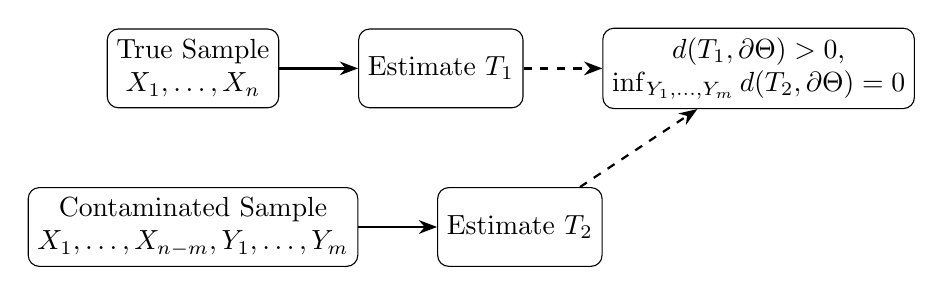
\begin{tikzpicture}[
        box/.style={draw, rounded corners, minimum width=2cm, minimum height=1cm, align=center},
        arrow/.style={-Stealth, thick},
        dashedarrow/.style={-Stealth, thick, dashed}
    ]
    % Nodes
    \node[box] (true) {True Sample \\ $X_1, \ldots, X_n$};
    \node[box, below=of true] (contaminated) {Contaminated Sample \\ $X_1, \ldots, X_{n-m}, Y_1, \ldots, Y_m$};    
    \node[box, right=of true] (T1) {Estimate $T_1$};
    \node[box, right=of contaminated] (T2) {Estimate $T_2$};    
    \node[box, right=of T1] (diff) { $d(T_1, \partial\Theta) > 0$, \\ $\inf_{Y_1,\dots, Y_m} d(T_2,\partial\Theta) = 0$};
    
    % Arrows
    \draw[arrow] (true) -- (T1);
    \draw[arrow] (contaminated) -- (T2);
    \draw[dashedarrow] (T1) -- (diff);
    \draw[dashedarrow] (T2) -- (diff);
    
    \end{tikzpicture}
\end{frame}


\begin{frame}{Robustness of Generalized Alpha-Beta Divergence}
    \begin{enumerate}
        \item Classical M-estimators have an asymptotic breakdown point at $1/(p+1)$. (\textcolor{blue}{Rousseeuw, 1985}).
        \pause
        \begin{tcolorbox}[colback=green!5!white,colframe=green!75!black]
        Given a model family of densities $\{ f_\theta \}$ and data density $g$, the minimum GAB divergence functional is 
        \begin{equation*}
            T_{MGABD}(G) = \argmin_{\theta \in \Theta} d_{GAB}^{(\alpha,\beta),\psi}(f_\theta, g)
        \end{equation*}
         \end{tcolorbox}
        \item Asymptotic BP of MGABD functional at location model is $1/2$.
        \pause
        \item Under suitable assumptions, asymptotic breakdown point is atleast
        \begin{equation*}
            \resizebox{0.9\hsize}{!}{%
            $\min\left\{ \liminf_{d(\theta_m,\partial\Theta) \rightarrow 0} \left[\frac{\psi^{-1}\left( \frac{\alpha}{\alpha+\beta}\psi(\int f_{\theta_m}^{\alpha+\beta})\right) }{ \int f_{\theta_m}^{\alpha+\beta} }\right]^{1/\beta}, 1 - \left[\frac{\psi^{-1}\left(\frac{\alpha}{\alpha+\beta} \psi(\int f_{\theta^g}^{\alpha+\beta}) \right) }{\int f_{\theta^g}^\alpha g^\beta }\right]^{1/\beta} \right\}$%
            }
        \end{equation*}
        \noindent In many cases with $\psi(x) = x$, this is $\left( \frac{\alpha}{\alpha+\beta} \right)^{1/\beta}$. 
    \end{enumerate}
\end{frame}

\begin{frame}{Asymptotic Distribution of MGABDE}
    \begin{enumerate}
        \item When $\beta = 1$, the MGABDE is an M-estimator with data-dependent $\psi_M(\cdot)$ or $\rho_M(\cdot)$ functions. 
        \item As a result, typical consistency and asymptotic normality holds as
        \begin{equation*}
            \sqrt{n}(\widehat{\theta}_n - \theta) \xrightarrow{d} N(0, V)
        \end{equation*}
        \begin{equation*}
            V = \frac{N_{1+2\alpha} - M_{1+\alpha}^2}{\left\vert N_{1+\alpha} + M_{1+\alpha}^2 \textcolor{blue}{\frac{\psi''(L_{1+\alpha})}{\psi'(L_{1+\alpha})}} \right\vert^2}            
        \end{equation*}
        \noindent where 
        \begin{equation*}
            L_{1+\alpha} = \int f_{\theta^g}^{1+\alpha}, \ M_{1+\alpha} = \int f_{\theta^g}^{1+\alpha}u_{\theta^g}, \ N_{1+\alpha} = \int f_{\theta^g}^{1+\alpha} u_{\theta^g}u_{\theta^g}\tr
        \end{equation*}
        \item This means, given a model family $f_\theta$, possible to find $\psi(\cdot)$ function that achieves optimal efficiency.
    \end{enumerate}

\end{frame}






\begin{frame}[shrink=20]
\frametitle{References}
    \begin{thebibliography}{9}
    \bibitem{basu1998robust} Basu, Ayanendranath, et al. "Robust and efficient estimation by minimising a density power divergence." Biometrika 85.3 (1998): 549-559.
    \bibitem{jones2001comparison} Jones, M. C., et al. "A comparison of related density-based minimum divergence estimators." Biometrika (2001): 865-873.
    \bibitem{kuchibhotla2019bridge} Kuchibhotla, Arun Kumar, Somabha Mukherjee, and Ayanendranath Basu. "Statistical inference based on bridge divergences." Annals of the Institute of Statistical Mathematics 71 (2019): 627-656.
    \bibitem{sdiv} Ghosh, Abhik, and Ayanendranath Basu. "The minimum S-divergence estimator under continuous models: The Basu–Lindsay approach." Statistical Papers 58 (2017): 341-372.
    \bibitem{maji2016logarithmic} Maji, Avijit, Abhik Ghosh, and Ayanendranath Basu. "The logarithmic super divergence and asymptotic inference properties." AStA Advances in Statistical Analysis 100 (2016): 99-131.
    \end{thebibliography}
\end{frame}



{\setbeamercolor{palette primary}{fg=ag-blue, bg=ag-beige}
\begin{frame}[standout]
  Thank you! \\
  Questions?
\end{frame}
}


\end{document}
